% Options for packages loaded elsewhere
\PassOptionsToPackage{unicode}{hyperref}
\PassOptionsToPackage{hyphens}{url}
\PassOptionsToPackage{dvipsnames,svgnames*,x11names*}{xcolor}
%
\documentclass[
  11pt,
  a4paper,
]{article}
\usepackage[]{mathpazo}
\usepackage{setspace}
\usepackage{amsmath}
\usepackage{ifxetex,ifluatex}
\ifnum 0\ifxetex 1\fi\ifluatex 1\fi=0 % if pdftex
  \usepackage[T1]{fontenc}
  \usepackage[utf8]{inputenc}
  \usepackage{textcomp} % provide euro and other symbols
  \usepackage{amssymb}
\else % if luatex or xetex
  \usepackage{unicode-math}
  \defaultfontfeatures{Scale=MatchLowercase}
  \defaultfontfeatures[\rmfamily]{Ligatures=TeX,Scale=1}
\fi
% Use upquote if available, for straight quotes in verbatim environments
\IfFileExists{upquote.sty}{\usepackage{upquote}}{}
\IfFileExists{microtype.sty}{% use microtype if available
  \usepackage[]{microtype}
  \UseMicrotypeSet[protrusion]{basicmath} % disable protrusion for tt fonts
}{}
\makeatletter
\@ifundefined{KOMAClassName}{% if non-KOMA class
  \IfFileExists{parskip.sty}{%
    \usepackage{parskip}
  }{% else
    \setlength{\parindent}{0pt}
    \setlength{\parskip}{6pt plus 2pt minus 1pt}}
}{% if KOMA class
  \KOMAoptions{parskip=half}}
\makeatother
\usepackage{xcolor}
\IfFileExists{xurl.sty}{\usepackage{xurl}}{} % add URL line breaks if available
\IfFileExists{bookmark.sty}{\usepackage{bookmark}}{\usepackage{hyperref}}
\hypersetup{
  pdftitle={Monte Carlo Simulation Applied on Discounted Cash Flow},
  pdfauthor={Francisco Piccolo},
  colorlinks=true,
  linkcolor=RoyalBlue,
  filecolor=Maroon,
  citecolor=Blue,
  urlcolor=RoyalBlue,
  pdfcreator={LaTeX via pandoc}}
\urlstyle{same} % disable monospaced font for URLs
\usepackage[margin=1in]{geometry}
\usepackage{longtable,booktabs}
\usepackage{calc} % for calculating minipage widths
% Correct order of tables after \paragraph or \subparagraph
\usepackage{etoolbox}
\makeatletter
\patchcmd\longtable{\par}{\if@noskipsec\mbox{}\fi\par}{}{}
\makeatother
% Allow footnotes in longtable head/foot
\IfFileExists{footnotehyper.sty}{\usepackage{footnotehyper}}{\usepackage{footnote}}
\makesavenoteenv{longtable}
\usepackage{graphicx}
\makeatletter
\def\maxwidth{\ifdim\Gin@nat@width>\linewidth\linewidth\else\Gin@nat@width\fi}
\def\maxheight{\ifdim\Gin@nat@height>\textheight\textheight\else\Gin@nat@height\fi}
\makeatother
% Scale images if necessary, so that they will not overflow the page
% margins by default, and it is still possible to overwrite the defaults
% using explicit options in \includegraphics[width, height, ...]{}
\setkeys{Gin}{width=\maxwidth,height=\maxheight,keepaspectratio}
% Set default figure placement to htbp
\makeatletter
\def\fps@figure{htbp}
\makeatother
\setlength{\emergencystretch}{3em} % prevent overfull lines
\providecommand{\tightlist}{%
  \setlength{\itemsep}{0pt}\setlength{\parskip}{0pt}}
\setcounter{secnumdepth}{-\maxdimen} % remove section numbering
\pagestyle{plain}
\usepackage{lineno} % add 

% Allowing for landscape pages
\usepackage{lscape}
\newcommand{\blandscape}{\begin{landscape}}
\newcommand{\elandscape}{\end{landscape}}

% Left justification of the text: see https://www.sharelatex.com/learn/Text_alignment
% \usepackage[document]{ragged2e} % already in the latex template
\newcommand{\bleft}{\begin{flushleft}}
\newcommand{\eleft}{\end{flushleft}}
\ifluatex
  \usepackage{selnolig}  % disable illegal ligatures
\fi

\title{Monte Carlo Simulation Applied on Discounted Cash Flow}
\author{Francisco Piccolo}
\date{}

\begin{document}
\maketitle

\setstretch{1.2}
\normalsize

\vspace{1cm}
\hrule

My abstract.

\vspace{3mm}
\hrule
\vspace{5mm}

\emph{Keywords}: My Keywords

\bleft
\newpage

\hypertarget{introduction}{%
\section{INTRODUCTION}\label{introduction}}

Write your introduction here. You can cite bibliography like this {[}@Yan2011; @Sutherland2011{]} if you provide a \texttt{BibTeX} file with references. See \url{http://rmarkdown.rstudio.com} for more information. Or you could also use \href{https://cran.r-project.org/web/packages/knitcitations/index.html}{knitcitations} or \href{https://cran.r-project.org/web/packages/RefManageR/index.html}{RefManageR} to fetch bibliographic metadata automatically from the web. For example, citing a paper can be as easy as providing its DOI.

You can even specify the desired output format for your bibliography by including a style file for a specific journal (e.g.~``ecology.csl''). Many different bibliography styles (CSL files) can be obtained at \url{http://citationstyles.org/}, \url{https://github.com/citation-style-language/styles}, or \url{https://zotero.org/styles}.

\hypertarget{methods}{%
\section{METHODS}\label{methods}}

\hypertarget{study-area}{%
\subsection{Study Area}\label{study-area}}

We worked in a \textbf{beautiful} place with lots of trees, like \emph{Quercus suber} and \emph{Laurus nobilis}.

\hypertarget{data-collection-and-analysis}{%
\subsection{Data collection and analysis}\label{data-collection-and-analysis}}

We applied a linear model where

\[
y_{i} = \alpha + \beta*x_{i} 
\]

\hypertarget{results}{%
\section{RESULTS}\label{results}}

Trees in forest \emph{A} grew taller than those in forest \emph{B} (mean height: 25 versus 13 m).

And many more cool results that get updated dynamically, e.g.~see Table \ref{tab:Table-mtcars} and Fig. \ref{fig:scatterplot}. Note Tables and Figures are cross-linked and numbered automatically. They could also appear in the middle of the document, not necessarily at the end.

\hypertarget{discussion}{%
\section{DISCUSSION}\label{discussion}}

Discuss.

\hypertarget{conclusions}{%
\section{CONCLUSIONS}\label{conclusions}}

Wrap up

\eleft

\clearpage

\listoftables

\newpage

\clearpage

\clearpage

\listoffigures

\begin{figure}

{\centering 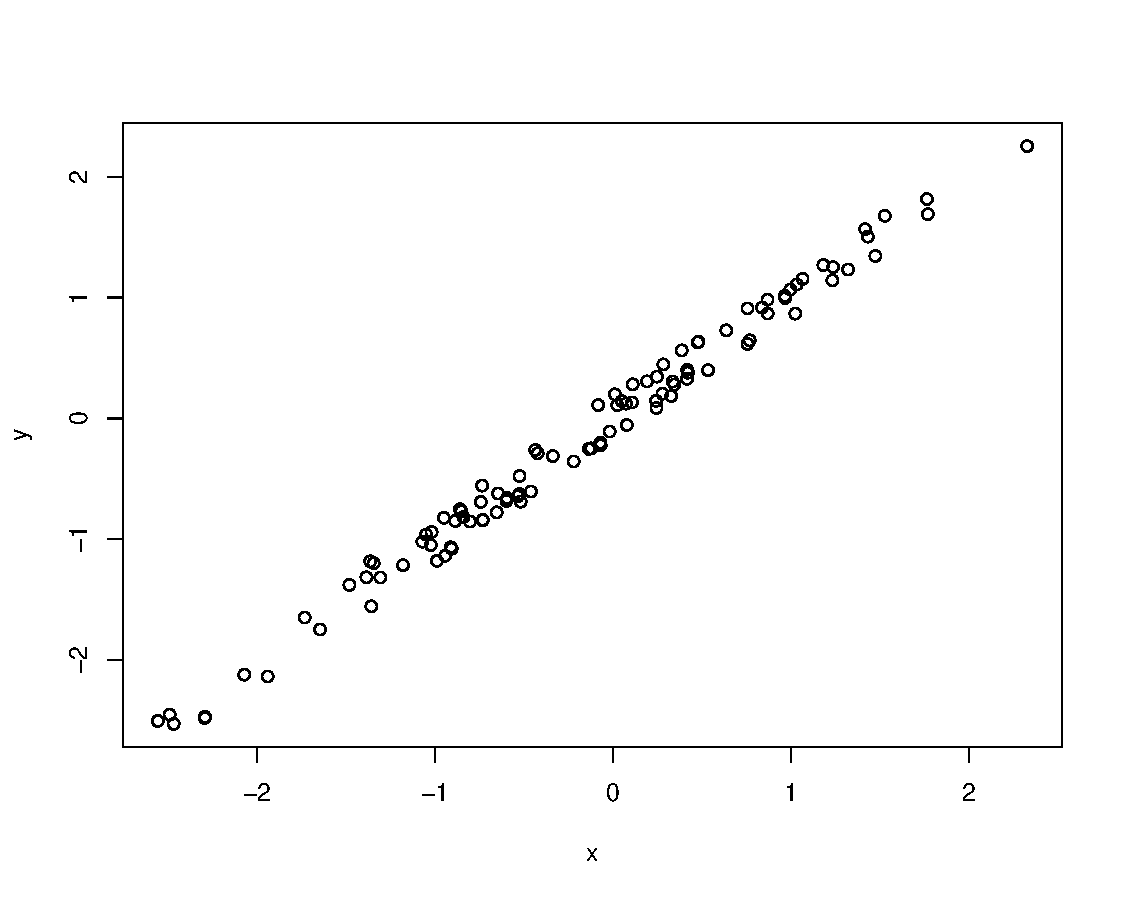
\includegraphics{output/figures/scatterplot-1} 

}

\caption{Just my first figure with a very fantastic caption.}\label{fig:scatterplot}
\end{figure}

\newpage

\end{document}
